\documentclass{standalone}
\begin{document}
\subsection{Aufgabe 10.3}
Skizze: \begin{center}
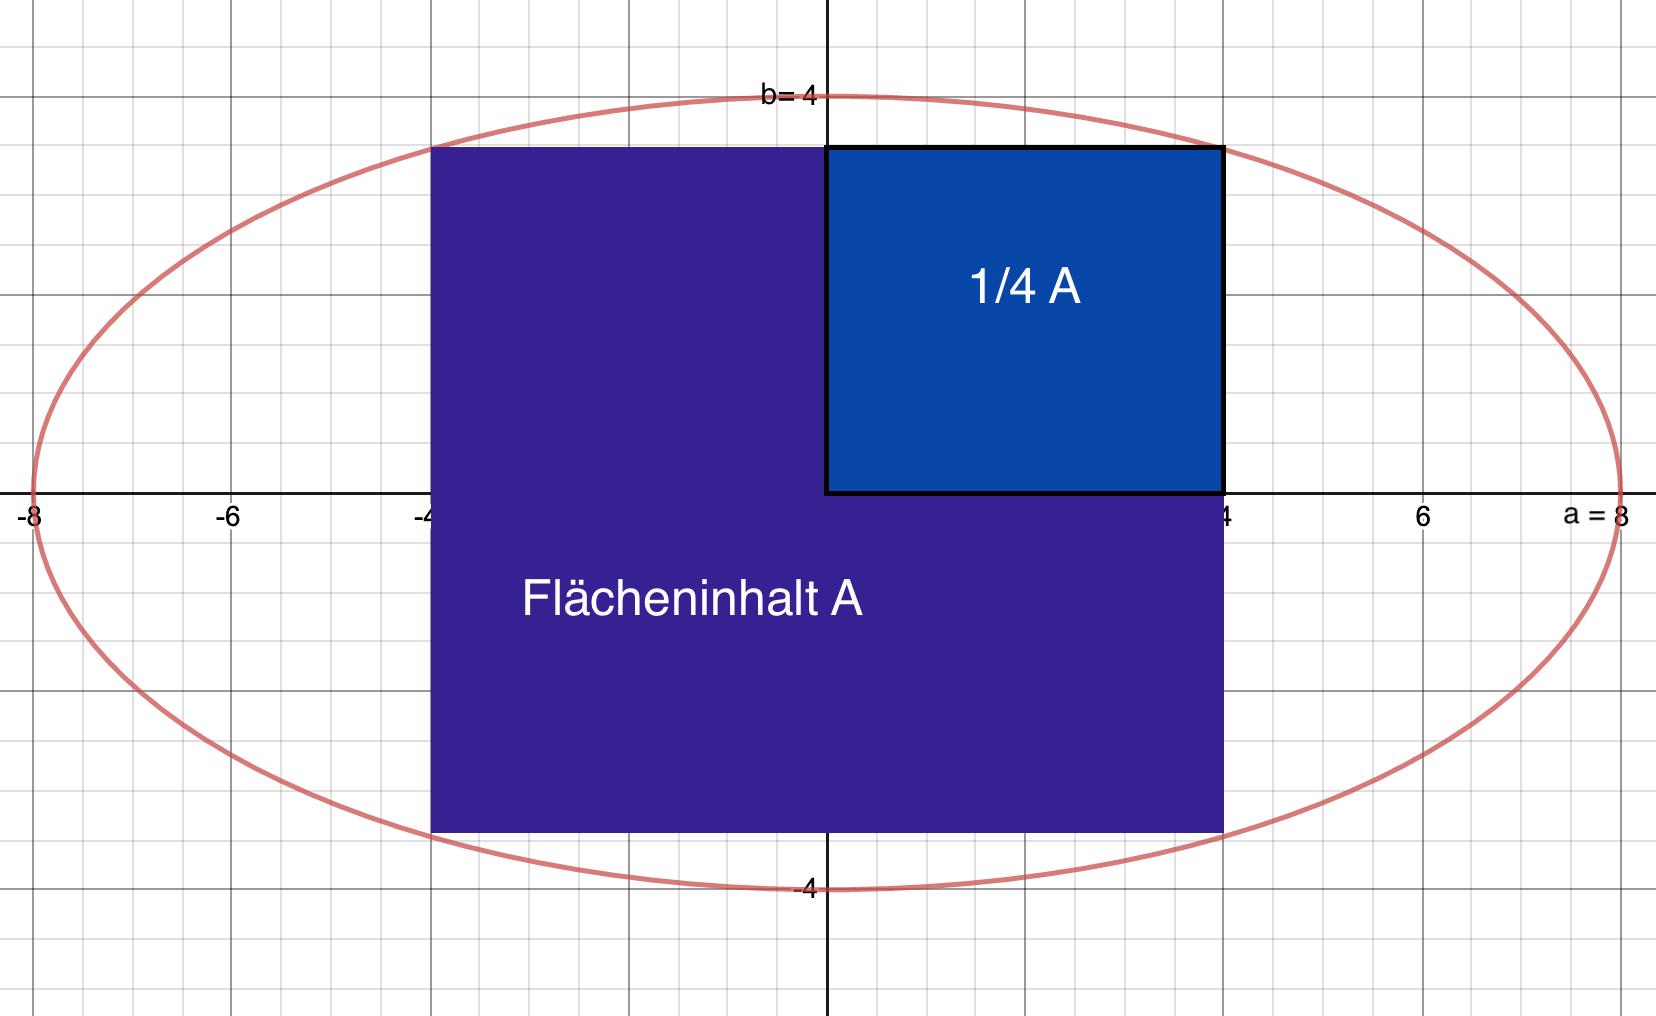
\includegraphics[width=11cm]{img/uebung10_a3.png}\end{center}
\begin{align}
F(x) &= \frac{b}{a} a \sqrt{a^2 - x^2} \\
F'(x) &= \frac{b}{a} \sqrt{a^2 - x^2} + \frac{1}{2}\frac{-2x \frac{b}{a}x}{\sqrt{a^2 -x^2}} = 0 \\
0 &= \frac{\frac{b}{a} (a^2 - x^2) - x^2 \frac{b}{a}}{\sqrt{a^2 - x^2}} \\
0 &=ba - \frac{b}{a} x^2 - \frac{b}{a} x^2 \\
ba &= 2 \frac{b}{a} x^2 \\
\frac{a^2}{2} &= x^2 \\
\frac{a}{\sqrt{2}} &= x
\end{align}
Dieser $x$-Wert muss dem globalen Hochpunkt entsprechen, da das Rechteck an den Randwerten von $x$ ($x = a$ und $x = 0$) einen Flächeninhalt von $0$ hat.

Seitenlängen $u$ (horizontal) und $v$ (vertikal):
\begin{align}
u &= 2x = 2 \frac{a}{\sqrt{2}} \\
v &= 2y
\end{align}
$x$ eingesetzt in $(\frac{x}{a})^2 + (\frac{y}{b})^2 = 1$ und nach y umgeformt:
\begin{align}
y &= b \frac{1}{\sqrt{2}} \\
v &= \frac{2}{\sqrt{2}} b \\
A_{Rechteck} &= 2 \frac{a}{\sqrt{2}} b \frac{2}{\sqrt{2}} \\
A_{Rechteck} &= 2ab
\end{align}
\end{document}